\section{Application specification}
\label{sec:app:specification}

To have an adequate base for application level testing of our protocol we restrict our application to the following requirements given in section \ref{sec:app:specification:req} \nameref{sec:app:specification:req}.\\

\subsection{Requirements}
\label{sec:app:specification:req}

\begin{req}
\label{req:app:load}
\textbf{bus load}: the application has to give us the ability to adjust the bus load rate to make exhaustive testing possible.
\end{req}

\begin{req}
\label{req:app:fault_injection}
\textbf{fault injection}: the application has to give us the ability to inject faulty transmissions in the time as well as in the value domain to test fault and error detection and correction.
\end{req}

\begin{req}
\label{req:app:message_loss}
\textbf{message loss}: the application has to give us the ability to detect message losses under ``normal'' conditions as well as in ``overload'' conditions.
\end{req}

% This is meant to be the pendant of an electro magnetic disturbance
% injected into the bus cable and should be detected through the
% CRC sums by the receiver.

\begin{req}
\label{req:app:sync_under_overloads}
\textbf{synchronization (drift rates) under overloads}: the application has to give us the ability to monitor drift rates of the clocks under heavy bus loads to evaluate the clock synchronization.
\end{req}

% That means that we are measuring:
% \begin{itemize}
%  \item The ability of the nodes to synchronize the clocks via the bus 
% while it is under load due to the bus load application
%  \item The drifts between the clocks before synchronizing
% \end{itemize}

\begin{req}
\label{req:app:visualization}
\textbf{visualization}: the application has to give us the ability to visualize drift rates and message losses via a graphical interface.
\end{req}

\begin{req}
\label{req:app:debug_and_monitor}
\textbf{Debugging and Monitoring features via PC}: The ability to debug through the PC is one of the first feature most developers are looking for. Therefore, it is a fundamental requirement for us to provide a bridging with respect to bus communication of the network nodes to a pc.
\end{req}


\subsection{Application design}
\label{sec:app:specification:design}

To give a short overview to the environment we use the four nodes of our microcontroller network as shown in figure \ref{fig:app:specification:node_overview} \nameref{fig:app:specification:node_overview} 
and outline the functionalities provided by the single nodes useful for our application level.\\

\begin{figure}[h]
 \centering
 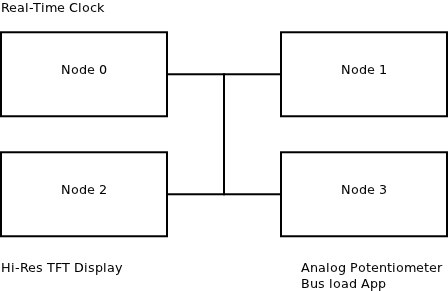
\includegraphics[scale=0.5]{../images/node_overview.png}
 % node_tasks.png: 448x291 pixel, 72dpi, 15.80x10.27 cm, bb=
 \caption{capabilities of nodes}
 \label{fig:app:specification:node_overview}
\end{figure}

\subsubsection{Node 0}
\label{sec:app:specification:node0}

Node 0 is used for standard communication purposes, messages are sent and received under certain predefined load conditions. Since the real time clock provided by the environment is
accessible by node 0 it is possible for some scenarios to synchronize the global time of the clock synchronization with the time of the real time clock.\\

For message loss measurements the task running on node 0 sends beside clock synchronization messages only messages holding a node specific counter incremented after every send attempt.\\ 

\subsubsection{Node 1}
\label{sec:app:specification:node1}

Node 1 is used for standard communication purposes, messages are sent and received under certain predefined load conditions.\\

For message loss measurements the task running on node 1 sends beside clock synchronization messages only messages holding 
a node specific counter incremented after every send attempt.\\ 

Besides the usecases depicted above, node 1 provides a push-button interface triggering transmissions of faulty messages 
by toggling single bits after the checksum calculation and another push-button interface to trigger synchronization messages 
simulating faulty messages in the time domain.\\

\subsubsection{Node 2}
\label{sec:app:specification:node2}

Node 2 is used to provide monitoring services via the LCD. For this purpose no filtering of messages is provided by the protocol.
All messages crossing the bus are stored and evaluated to certain properties such as

\begin{enumerate}
 \item the drifts of the certain clocks
 \item message loss rates
\end{enumerate}

and can be visualized via the LCD as pure text or as chart.\\

Although node 2 has a fully CNI (communication network interface) available the only messages transmitted by node 2 are messages for synchronization purposes and debug messages.\\

A sketch how the visualization could look is given in figure \ref{fig:app:specification:node2} \nameref{fig:app:specification:node2}.

\begin{figure}[h]
 \centering
 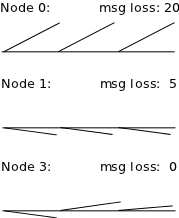
\includegraphics[scale=0.8]{../images/app_visu_sketch.png}
 % node_tasks.png: 448x291 pixel, 72dpi, 15.80x10.27 cm, bb=
 \caption{sketch of visualization}
 \label{fig:app:specification:node2}
\end{figure}


\subsubsection{Node 3}
\label{sec:app:specification:node3}

Node 3 is used for standard communication purposes, messages are sent and received under certain load conditions.\\

Since node 3 can access the value of the analog potentiometer the task for node 3 is to increase or decrease the bus load by sending or leaving out messages according to the value adjusted by the potentiometer.\\

For message loss measurements the task running on node 3 sends beside clock synchronization messages only messages holding a node specific counter incremented after every send attempt.\\ 
